\documentclass[11pt]{beamer}
\usetheme{Frankfurt}
\usepackage[latin1]{inputenc}
\usepackage[T1]{fontenc}
\usepackage{appendixnumberbeamer}

\usepackage{multirow}

\usepackage{hyperref}

\usepackage{tikz}

\usetikzlibrary{arrows, backgrounds, positioning, fit, matrix}

\usepackage{gitdags}

\usepackage{listings}

\newcommand\Small{\fontsize{8}{8.0}\selectfont}
\newcommand*\LSTfont{\Small\ttfamily}

\lstset{
    basicstyle=\LSTfont,
    backgroundcolor=\color{white},
    showspaces=false,
    showstringspaces=false,
    showtabs=false,
    rulecolor=\color{black},
    tabsize=4,
    breaklines=true,
    keywordstyle=\color{blue},
    commentstyle=\color{gray},
    stringstyle=\color{orange}
}

\title{Introduction into Git}
%\author{}<++>

\date{\today}

\begin{document}

\maketitle

\section{Version Control Systems}

\begin{frame}[fragile]{What is Git?}

    \emph{Git is a decentralized VCS (Version Control System).}

    \begin{figure}
        \centering
        
\includegraphics[height=0.6\textheight]{img/xkcdgit.png}
        \caption{\textit{https://xkcd.com/1597/}}
    \end{figure}

\end{frame}

\begin{frame}[fragile]{Why Git?}

    \begin{figure}
        \centering
        
\includegraphics[height=0.6\textheight]{img/does_not_simply.png}
    \end{figure}

\end{frame}

\begin{frame}[fragile]{Version Control Systems}
    \emph{Local Version Control System}
    \vspace{1cm}

    \begin{minipage}{0.49\textwidth}
        \begin{itemize}
            \item store different versions of a file
            \item simple but error prone
            \item \emph{rcs} - Revsion control system
        \end{itemize}
    \end{minipage}
    \begin{minipage}{0.49\textwidth}
    \begin{figure}
        \centering
        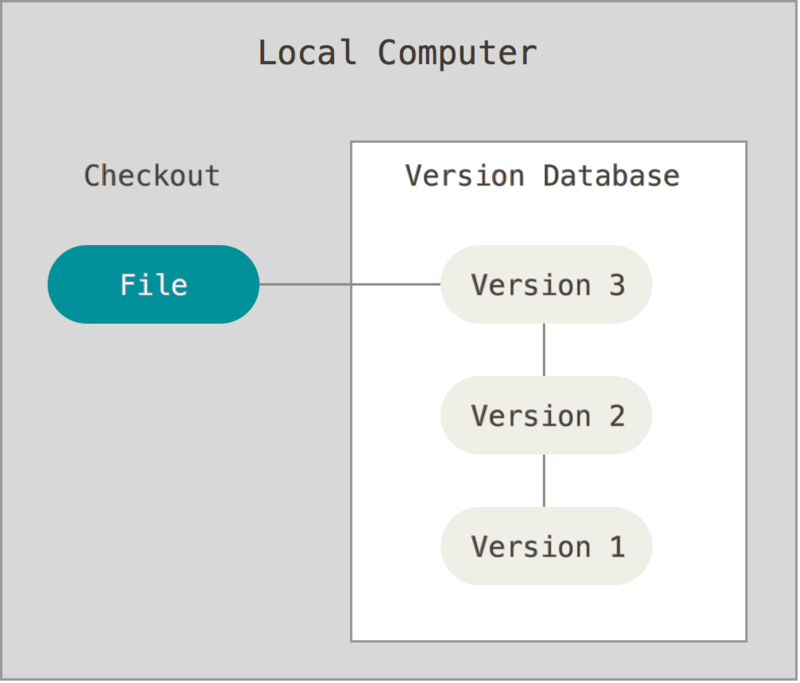
\includegraphics[width=0.9\textwidth]{img/local_vcs.png}
    \end{figure}
    \end{minipage}

\end{frame}

\begin{frame}[fragile]{Version Control System}
    \emph{Centralized Version Control Systems}
    \vspace{1cm}

    \begin{minipage}{0.49\textwidth}
        \begin{itemize}
            \item single server that conatins all the versioned files
            \item clients check out files from that central place
            \item single point of failure
            \item \emph{Subversion}, \emph{CVS}
        \end{itemize}
    \end{minipage}
    \begin{minipage}{0.49\textwidth}
        \begin{figure}
            \centering
            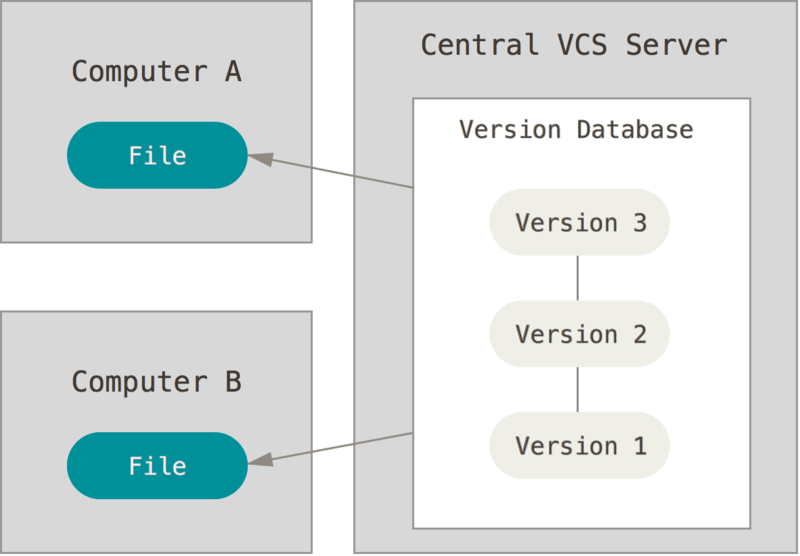
\includegraphics[width=0.9\textwidth]{img/centralized_vcs.png}
        \end{figure}
    \end{minipage}

\end{frame}

\begin{frame}[fragile]{Version Control System}
    \emph{Distributed Version Control System}
    \vspace{1cm}

    \begin{minipage}{0.49\textwidth}
        \begin{itemize}
            \item clients fully mirror the repository
            \item serveral remote repositories possible
            \item \emph{Git}, \emph{Mercurial}, \emph{Barzaar}
        \end{itemize}
    \end{minipage}
    \begin{minipage}{0.49\textwidth}
        \begin{figure}
            \centering
            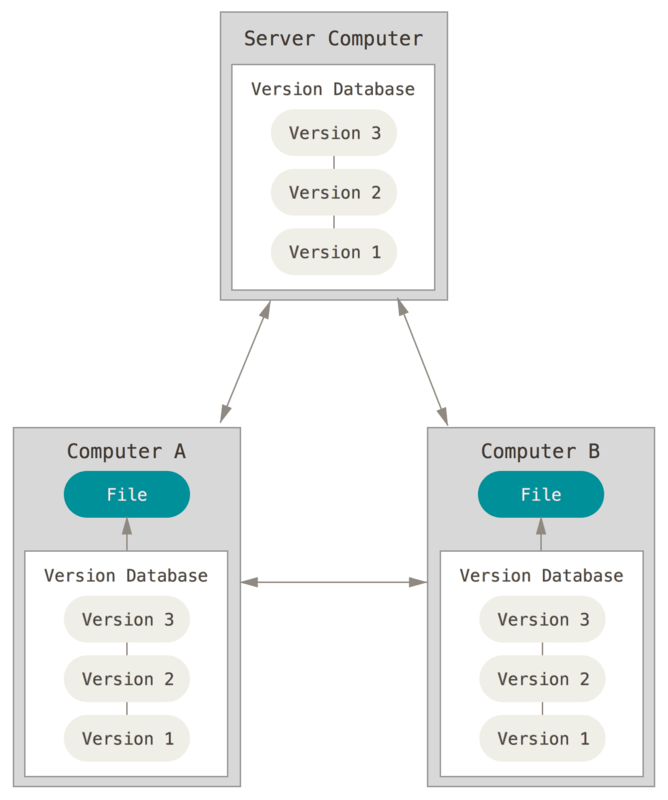
\includegraphics[width=0.9\textwidth]{img/distributed_vcs.png}
        \end{figure}
    \end{minipage}

\end{frame}

\section{Git Introduction}

\begin{frame}[fragile]{Installing git}

    \textbf{Debian:}
    \begin{lstlisting}
    apt install git
    \end{lstlisting}

    \textbf{Arch Linux:}
    \begin{lstlisting}
    pacman -S git
    \end{lstlisting}

    \textbf{Fedora:}
    \begin{lstlisting}
    dnf install git
    \end{lstlisting}

    \begin{description}
        \item{For Linux:} \url{http://git-scm.com/download/linux}
        \item{For Mac:} \url{http://git-scm.com/download/mac}
        \item{For Windows:} \url{http://git-scm.com/download/win}
    \end{description}

\end{frame}

\begin{frame}[fragile]{How it works}
    \begin{figure}
        \centering
        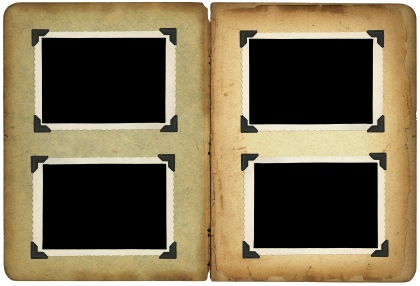
\includegraphics[width=0.8\textwidth]{img/photo_album.jpg}
        \caption{like a photo album of you work}
    \end{figure}
\end{frame}

\begin{frame}[fragile]{How it works}
    \begin{figure}
        \centering
        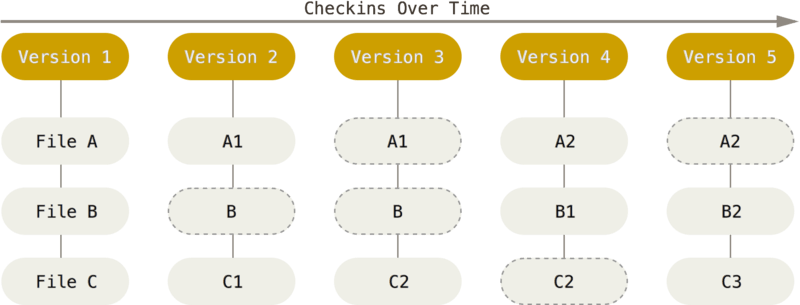
\includegraphics[width=0.8\textwidth]{img/snapshotbased.png}
        \caption{storing stream of snapshots over time}
    \end{figure}
\end{frame}

%\begin{frame}[fragile]{How it NOT works}
    %\begin{figure}
        %\centering
        %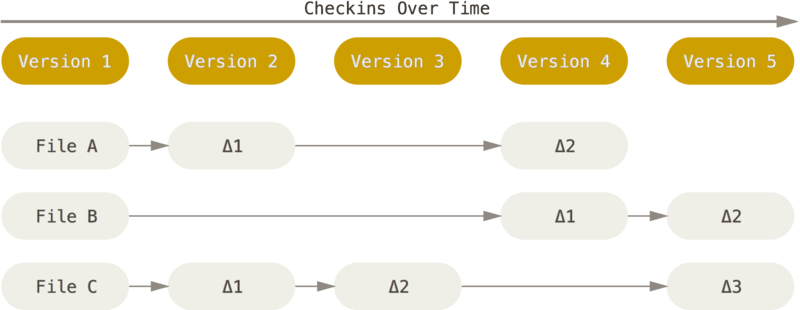
\includegraphics[width=0.8\textwidth]{img/filebased.png}
        %\caption{storing changes to a base file}
    %\end{figure}
%\end{frame}

\begin{frame}{What is a git repository?}

    \begin{figure}
        \centering
        \includegraphics[width=0.9\textwidth]{img/three_states.png}
    \end{figure}
\end{frame}

%\begin{frame}{Basic Workflow}
    %\begin{enumerate}
        %\item Modify files in your working directory.
        %\item Stage the files, adding snapshots of them to your staging area.
        %\item Commit, stores the snapshot in the staging area permanently in
            %your git directory.
        %\item Push your commits to an remote repository on a server.
    %\end{enumerate}
%\end{frame}

\defverbatim\setusername{%
    \scriptsize
    \verb+git config --global user.name "Max Mustermann"+
    \newline
}
\defverbatim\setusermail{%
    \scriptsize
    \verb+git config --global user.mail "max.mustermann@example.org"+
    \newline
}

%\begin{frame}{Configure Git}

    %\emph{Place where the git configuration can live:}
    %\vspace{1cm}

    %% TODO: take a table for that
    %\begin{itemize}
            %\item \textbf{/etc/gitconfig} system wide configuration
                %\textit{-\,-system}
            %\item \textbf{$\sim$/.gitconfig} or \textbf{$\sim$/.config/gitconfig}  user wide configuration \textit{-\,-global}
            %\item \textbf{.git/config} repository specific configuration
    %\end{itemize}

%\end{frame}

\begin{frame}[fragile]{Configure Git}
    \textbf{Show your configuration:}
    \begin{lstlisting}
        git config --list
    \end{lstlisting}
    \textbf{Show specific configuration value:}
    \begin{lstlisting}
        git config user.name
    \end{lstlisting}
    \textbf{Define an alias:}
    \begin{lstlisting}
        git config alias.st=git status
    \end{lstlisting}
    \textbf{Enable highlighting:}
    \begin{lstlisting}
        git config --global color.ui=always
    \end{lstlisting}
\end{frame}

\begin{frame}[fragile]{Setup Your Environment}
    \emph{Three essentail configuration values you should have set.}
    \vspace{1cm}

    \textbf{Your name:}
    \begin{lstlisting}
        git config --global user.name "Max Mustermann"
    \end{lstlisting}
    \textbf{Your email address:}
    \begin{lstlisting}
        git config --global user.mail "max@example.org"
    \end{lstlisting}
    \textbf{Your editor:}
    \begin{lstlisting}
        git config --global core.editor "vim"
    \end{lstlisting}
\end{frame}

\begin{frame}[fragile]{Lets Start\ldots}
    \textbf{Start from scratch:}
    \begin{lstlisting}
mkdir my_new_project
cd my_new_project
git init
    \end{lstlisting}
    \textbf{Get a local copy of a repository that already exist.}
    \begin{lstlisting}
git clone https://github.com/blastmaster/ta-git_intro.git
git clone -b <branchname> <GIT_URL>
    \end{lstlisting}
\end{frame}

%\begin{frame}[fragile]{Follow the changes}
    %\textbf{What is the status of your local repo?}
    %\begin{lstlisting}
        %git status
    %\end{lstlisting}
    %\textbf{What happens so far?}
    %\begin{lstlisting}
        %git log
    %\end{lstlisting}
    %\textbf{What has changed?}
    %\begin{lstlisting}
        %git diff [--staged]
    %\end{lstlisting}
    %\textbf{Who has changed?}
    %\begin{lstlisting}
        %git blame
    %\end{lstlisting}
%\end{frame}

%\begin{frame}[fragile]{Ignoring Files}
    %\emph{Ignore files that follow a specific pattern with a \textbf{.gitignore} file}

    %\textit{.gitignore} rules:
    %\begin{itemize}
        %\item Black lines or lines starting with \# are ignored.
        %\item Standard glob pattern work.
        %\item You can start patterns with a forward slash (/) to avoid recusivity.
        %\item You can negate a pattern by starting it with an exclamation point (!).
    %\end{itemize}

    %\vspace{1em}
    %Example:\\
    %\url{https://github.com/github/gitignore}

%\end{frame}

\section{Pitfalls}

\begin{frame}[fragile]{Oh shit, I did something terribly wrong, please tell me git has a magic time machine!?!}
    \begin{figure}
    \begin{lstlisting}
        git reflog
        # you will see a list of every thing you've done in git, across all branches!
        # each one has an index HEAD@{index}
        # find the one before you broke everything
        git reset HEAD@{index}
        # magic time machine
    \end{lstlisting}
    \end{figure}
\end{frame}

\begin{frame}[fragile]{Oh shit, I committed and immediately realized I need to make one small change!}
    \begin{figure}
    \begin{lstlisting}
        # make your change
        git add . # or add individual files
        git commit --amend
        # follow prompts to change or keep the commit message
        # now your last commit contains that change!
    \end{lstlisting}
    \end{figure}
\end{frame}

\begin{frame}[fragile]{Oh shit, I need to change the message on my last commit!}
    \begin{figure}
    \begin{lstlisting}
        git commit --amend
        # follow prompts to change the commit message
    \end{lstlisting}
    \end{figure}
\end{frame}

\begin{frame}[fragile]{Oh shit, I accidentally committed something to master that should have been on a brand new branch!}
    \begin{figure}
    \begin{lstlisting}
        # create a new branch from the current state of master
        git branch some-new-branch-name
        # remove the commit from the master branch
        git reset HEAD~ --hard
        git checkout some-new-branch-name
        # your commit lives in this branch now :)
    \end{lstlisting}
    \end{figure}
\end{frame}

\begin{frame}[fragile]{Oh shit, I accidentally committed to the wrong branch!}
    \begin{figure}
    \begin{lstlisting}
        # undo the last commit, but leave the changes available
        git reset HEAD~ --soft
        git stash
        # move to the correct branch
        git checkout name-of-the-correct-branch
        git stash pop
        git add . # or add individual files
        git commit -m "your message here"
        # now your changes are on the correct branch
        \end{lstlisting}
\end{figure}
\end{frame}

\begin{frame}[fragile]{Fuck this noise, I give up.}

    \begin{figure}
        \begin{lstlisting}
        cd ..
        rm -rf git-repo-dir
        git clone https://some.github.url/git-repo-dir.git
        cd git-repo-dir
        \end{lstlisting}
    \end{figure}
\end{frame}

\begin{frame}{End}

    \begin{figure}
    \centering
    
\includegraphics[width=\textwidth]{img/git-logo.png}
    \end{figure}

\end{frame}


\end{document}
